\documentclass[12pt, letterpaper]{article}
\usepackage{graphicx}
\usepackage[UTF8]{ctex}
\renewcommand{\figurename}{Fig}
\graphicspath{{images/}}
% \usepackage{xeCJK}
\title{Test Paper}
\author{HONG Xiao\thanks{Funded by myself}}
\date{Sep. 2024}
\begin{document}
\maketitle
% The comment will not be shown
\%this will be show
First Document. Try to write something. This is not the finish version.and... \LaTeX{}
\begin{figure}
    \centering
    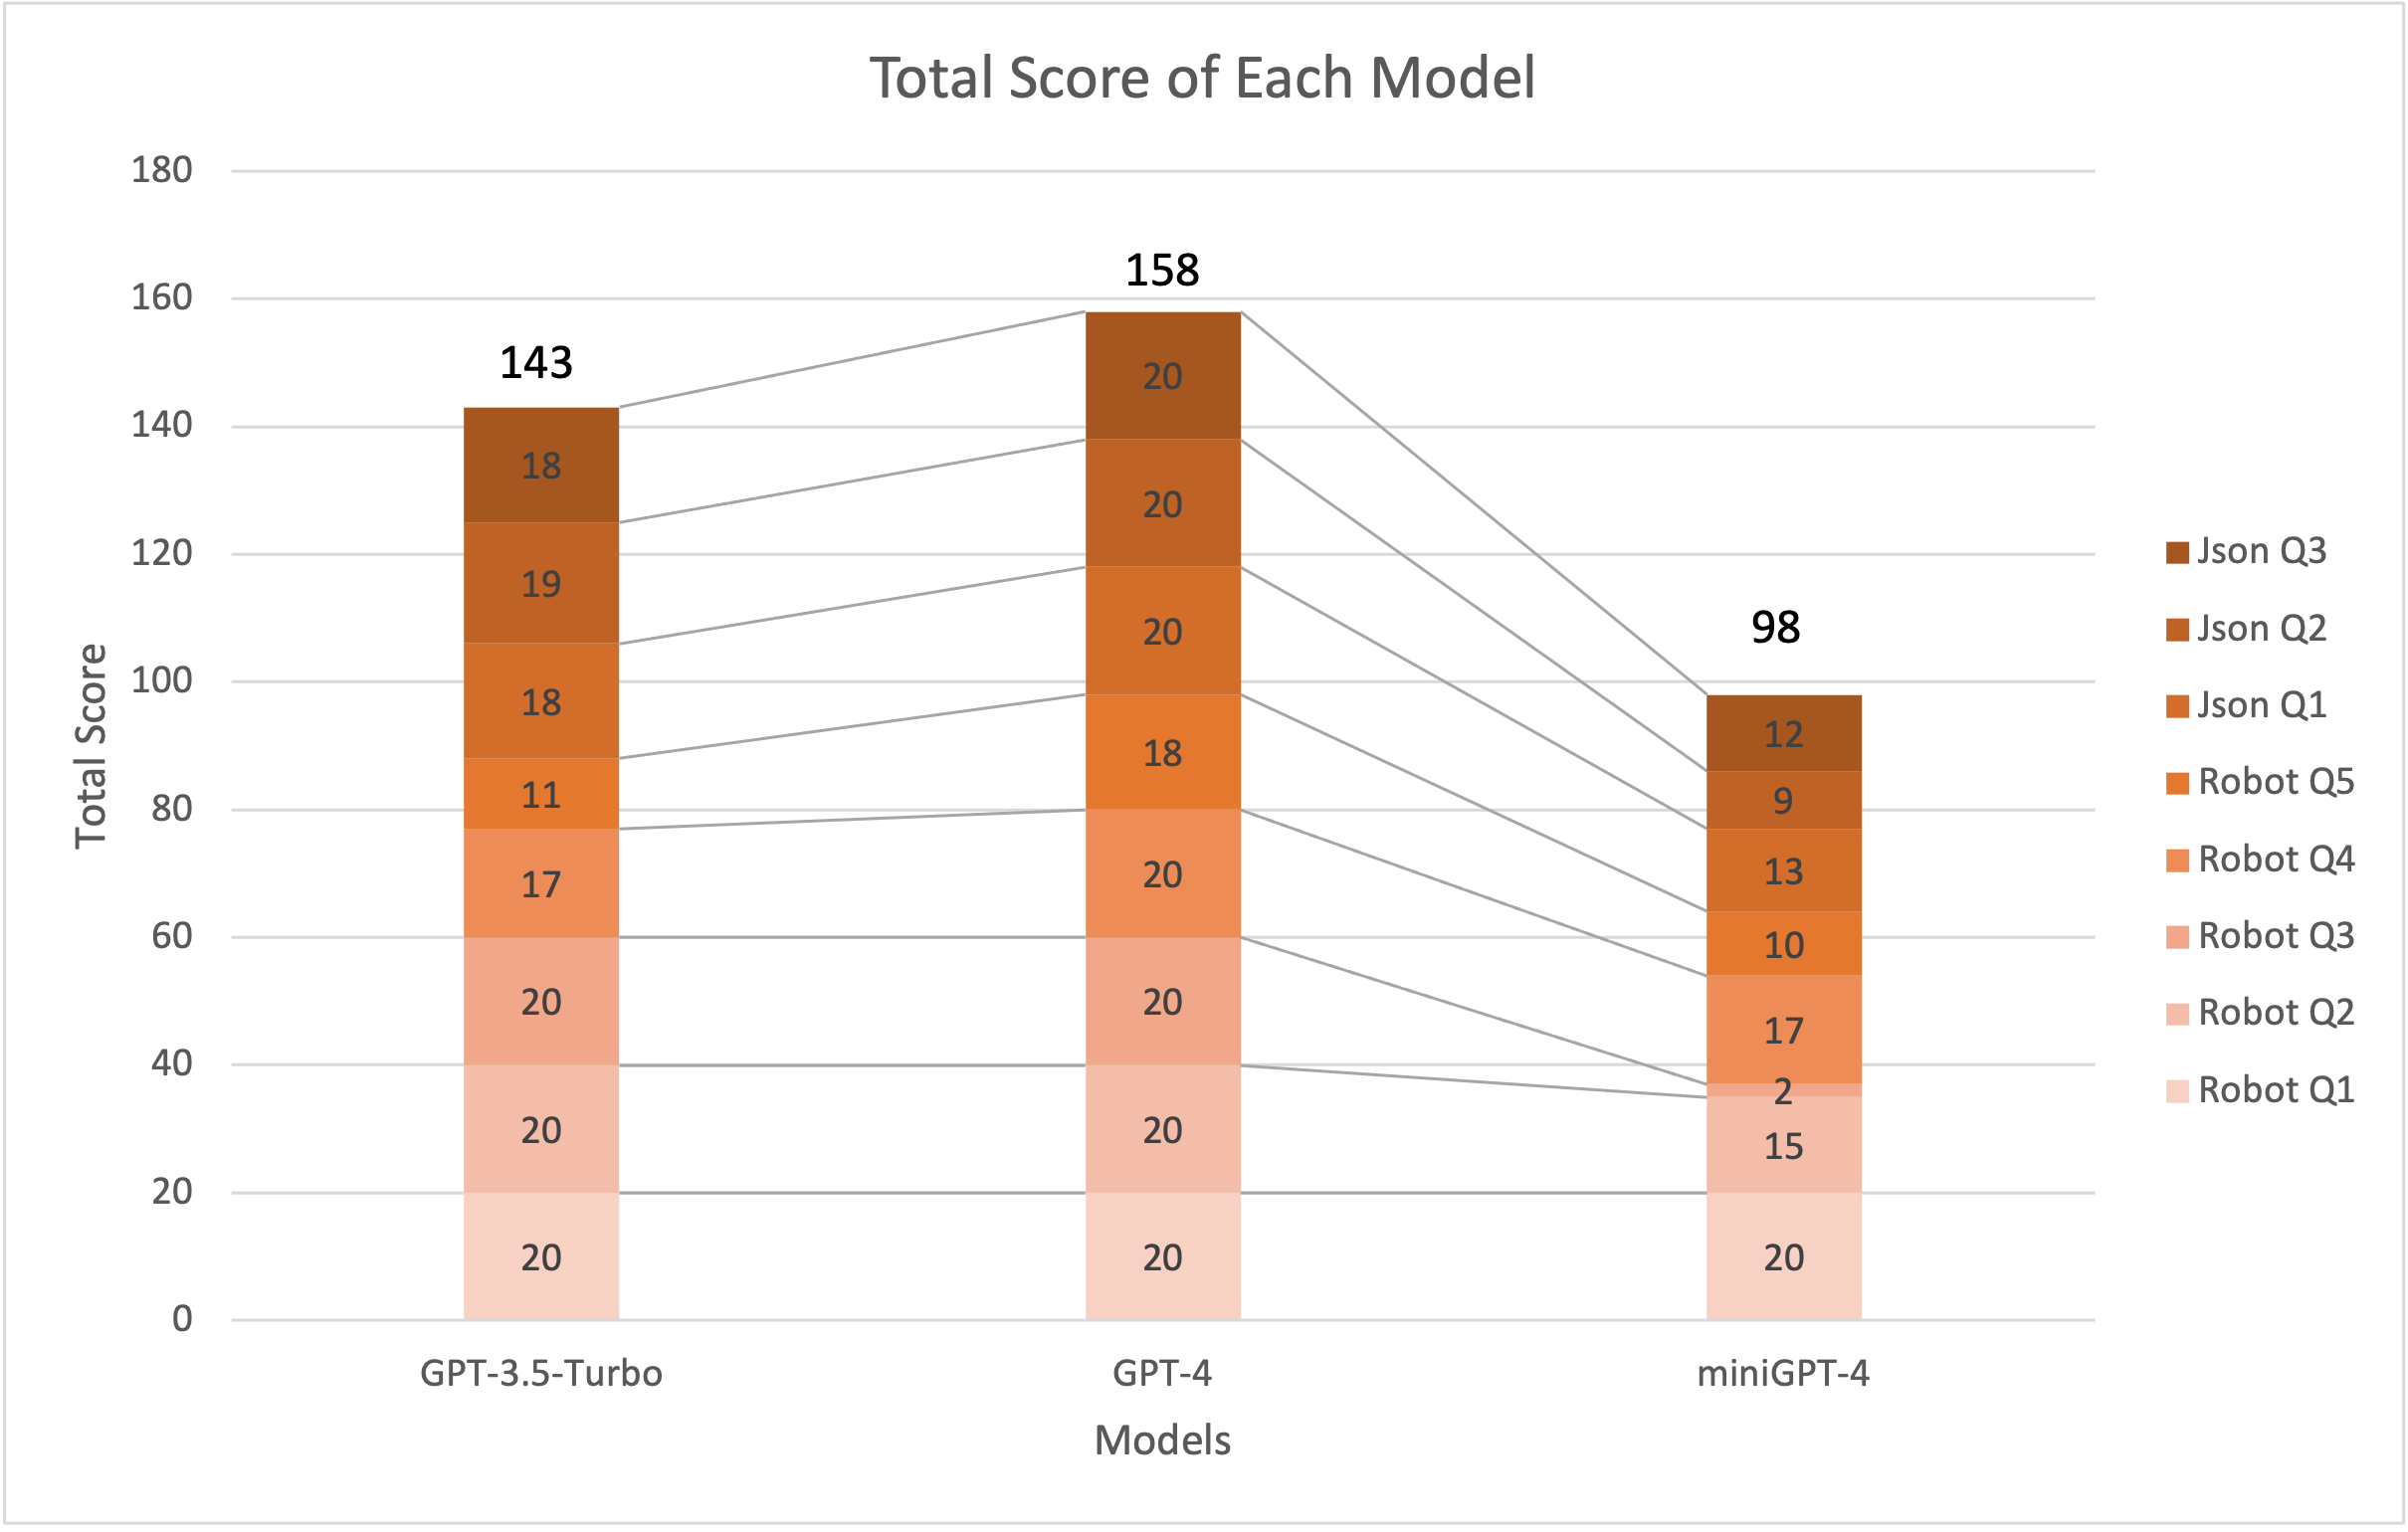
\includegraphics[width=0.75\textwidth]{scores_of_each_model}
    \caption{One of the exp}
    \label{Figure:34}
\end{figure}
Some of \textbf{bold} and some of \textit{italy\emph{is important}right?} and some of \underline{underline}

Usually, you need to use tow blank lines to return

such as this
and this will be at the same line
\end{document}